\documentclass{article}
\usepackage[utf8]{inputenc}
\usepackage{amsmath}
\usepackage{amsfonts}
\usepackage{graphicx}
\usepackage{todonotes}
\usepackage{hyperref}
\newcommand{\acc}{\text{acc}}
\newcommand{\conf}{\text{conf}}
\newcommand{\D}{\mathcal{D}}
\hypersetup{
    colorlinks=true,
    linkcolor=blue,
    filecolor=magenta,      
    urlcolor=blue,
    pdftitle={Overleaf Example},
    pdfpagemode=FullScreen,
}

\title{Calibration}

\begin{document}

\maketitle

\section{Introduction}
In high-stakes professions, in which there are large consequences for failure, it’s very important to have a good sense of your own uncertainty. Consider doctors or other medical practitioners. A wrong diagnosis or treatment could cost thousands of dollars or even lead to death. Given this, doctors need to know when to be confident in their own diagnosis and when to defer to a specialist or a second opinion. Having a good grasp of uncertainty as a doctor saves both lives and money. 

This property is even more important for machine learning systems in the medical domain. Such systems are often uninterpretable and make decisions in a manner which obfuscates the decision-making process. If doctors cannot make external judgments about when a system's reasoning is likely to fail, then the system itself must have a good sense of its confidence in each prediction. Otherwise, doctors may be deferential to the machine learning systems, even when the system is making an obvious mistake.

The property of knowing when you’re likely to fail is called `calibration.' More specifically, in classification tasks, a well-calibrated classifier provides accurate probability estimates on whether its answer is correct. In other words, a well-calibrated classifier has a good grasp of its uncertainty and is neither overconfident nor underconfident in its predictions. In 2017, researchers at Cornell discovered that large neural networks have progressively gotten worse at calibration over time \cite{guo2017calibration}. They compared LeNet, which consists of only 5 layers, and ResNet, which has 110 total layers. ResNet performed much better in predictive accuracy but was more poorly calibrated when compared to LeNet. Specifically, ResNet was consistently overconfident in its predictions. Similar patterns were shown in other ResNet-based models. Researchers begun trying to find ways to calibrate deep neural networks, thus creating the field of deep learning calibration.

\section{Problem Statement}
Formally, calibration is defined as follows. A classifier maps an input $x$ to a probability distribution over potential classes $p(y|x)$. Calibration involves ensuring that a model’s output probability distribution $p(y|x)$ matches the actual probability of a correct prediction. Say a model gives a 90\% confidence to a certain prediction. If the model is well-calibrated, then 90\% of the time, the prediction is correct. 

\subsection{Metrics}
To evaluate calibration, researchers commonly use four different metrics: expected calibration error, maximal calibration error, and negative log likelihood, and brier score. Expected calibration error is by far the most common, although the other metrics are also sometimes used.

\subsubsection{Expected Calibration Error}
Expected calibration error (ECE) is the primary metric for testing calibration \cite{naeini2015obtaining}. To calculate ECE, we first divide up the interval between 0 and 1 into bins. For instance, we might let the bins be [0, 0.1], [0.1, 0.2], … [0.9, 1]. Then we place examples into these bins based on the model’s confidence when making the prediction. Often this means taking the max of the model’s post-softmax prediction scores. Finally, we take the weighted sum of the absolute difference between the real accuracy and the predicted accuracy. The sum is weighted based on the number of examples in each bin. Formally, say we have $n$ examples partitioned up into $M$ bins $B_1, B_2, …, B_M$. Also, let $\acc(B_m)$ be the average accuracy of examples in the bin and let $\conf(B_m)$ be the average confidence of examples in the bin. Then ECE is defined as:

\[
    \text{ECE} = \sum_{m=1}^M\frac{|B_m|}{n}\left|\acc(B_m) - \conf(B_m)\right|
\]

\noindent ECE ranges between 0 and 1, with lower scores being better. What is considered a strong ECE varies from dataset to dataset. Reading a few papers, we get that ImageNet classifiers usually have ECE which varies from 0.01 to 0.08 and a score of 0.02 or lower can be considered strong \cite{guo2017calibration, minderer2021revisiting}.

\subsubsection{Maximum Calibration Error}
The Maximum Calibration Error (MCE) is similar to ECE but meant for much more sensitive domains \cite{naeini2015obtaining}. Like ECE, we partition the interval up into bins. However, instead of taking a weighted average of calibration score over bins, we take the maximum calibration error over bins. In other words MCE aims to reduce the calibration error of the worst bin, with the intuition that this prevents catastrophic failure cases while giving up some efficacy on more mundane cases. 

\[
    \text{MCE} = \max_{m \in \{1, ..., M\}}|\acc(B_m) - \conf(B_m)|
\]

\noindent Like ECE, MCE ranges between 0 and 1, with lower scores being better. MCE is much less common than ECE. Quickly eyeballing some results gives us that a model with an MCE of 0.1 can be considered strong \cite{guo2017calibration}.

\subsubsection{Negative Log Likelihood}
The likelihood of a dataset is the probability that a model assigns to the entire dataset. It is defined as follows: 

\[
    \text{Likelihood} = \prod_{x, y \sim \D} p(y|x)
\]

\noindent for $p(y|x)$ our classifier. For numerical stability reasons, it's common practice to take the negative log likelihood (NLL) defined as follows:

\[
    \text{NLL} = -\sum_{x,y \sim \D} \log p(y|x)
\]

\noindent Negative log likelihood (or cross-entropy loss) is commonly used for maximizing predictive accuracy. However, NLL is also useful for calibration as well; a classic result in statistics shows that NLL is minimized precisely when $p(y|x)$ matches the true probability distribution $\pi(y|x)$ \cite{hastie2009elements}. In other words, NLL is minimized at zero when the classifier is perfectly calibrated. In addition, a poor classifier can have unbounded NLL.

\subsubsection{Brier Score}
Finally, brier score is a common way to measure the accuracy of probability estimates, historically used in measuring forecasting accuracy \cite{brier1950verification}. It is equivalent to measuring the mean squared error of the probability, as follows. 

\[
    \text{Brier Score} = \frac{1}{|\D|} \sum_{x,y \sim \D}(y - f_\theta(x))^2
\]

\noindent Brier score is used in many real-world applications, such as assessing weather, sports, or political predictions. Brier score is a “strictly proper scoring rule,” meaning that one can uniquely maximize one’s score by predicting the true probabilities. Brier score ranges between 0 and 1, with an optimal model having a score of 0.

\subsection{Modern Neural Networks are Miscalibrated}
Now that we understand the definition of calibration error, we can revisit the researchers at Cornell \cite{guo2017calibration}. These researchers showed that ResNets were overconfident compared to LeNets, depicted visually in Figure \ref{fig:modern}. The top two plots show the histogram of confidences and the bottom two plots show the gap between the expected and actual accuracy for each bin. 

\begin{figure}
    \centering
    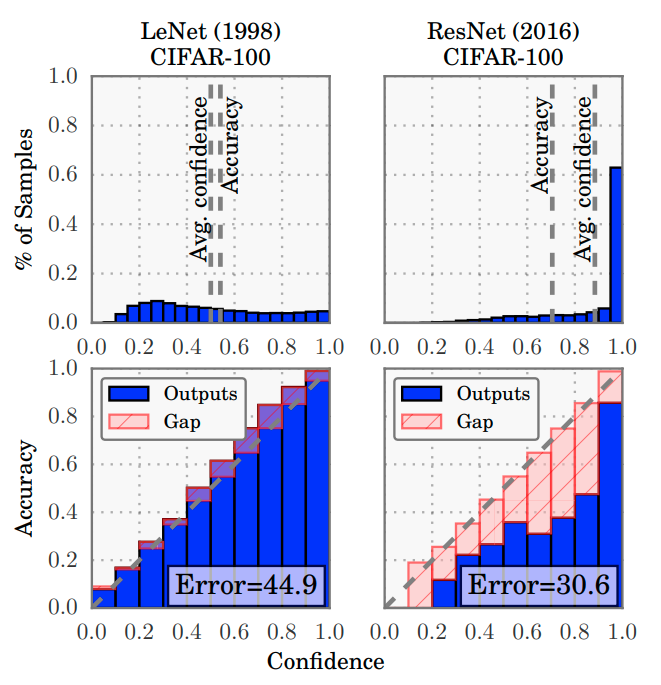
\includegraphics[width=7.5cm]{images/modern.png}
    \caption{The confidence histogram (top) and reliability diagram (bot) of a LeNet (left) and ResNet (right). Figure taken from \cite{guo2017calibration}.}
    \label{fig:modern}
\end{figure}

Notice how the confidence scores for ResNets are quite concentrated in the last bin and how the actual accuracy in each bin is much lower than the expected accuracy. Even though ResNets improved accuracy by 14.3 percentage points on Cifar100, calibration error increased from 0.0485 to between 0.1057 and 0.1653!

\section{Approaches}
\subsection{Temperature Scaling}

The same researchers from Cornell introduce “temperature scaling” which involves dividing the pre-softmax logits of a model by some constant T before applying softmax. Specifically, it is implemented as follows:

\[
    \text{softmax}(x, T) = \frac{\exp(x/T)}{\sum_i \exp(x_i/T)}
\]

\noindent The intuition here is that temperature controls how spread out the predictions are without modifying the predictions (and therefore the accuracy). See figure \ref{fig:temperature} for a visualization of this.

\begin{figure} % Logits?
    \centering
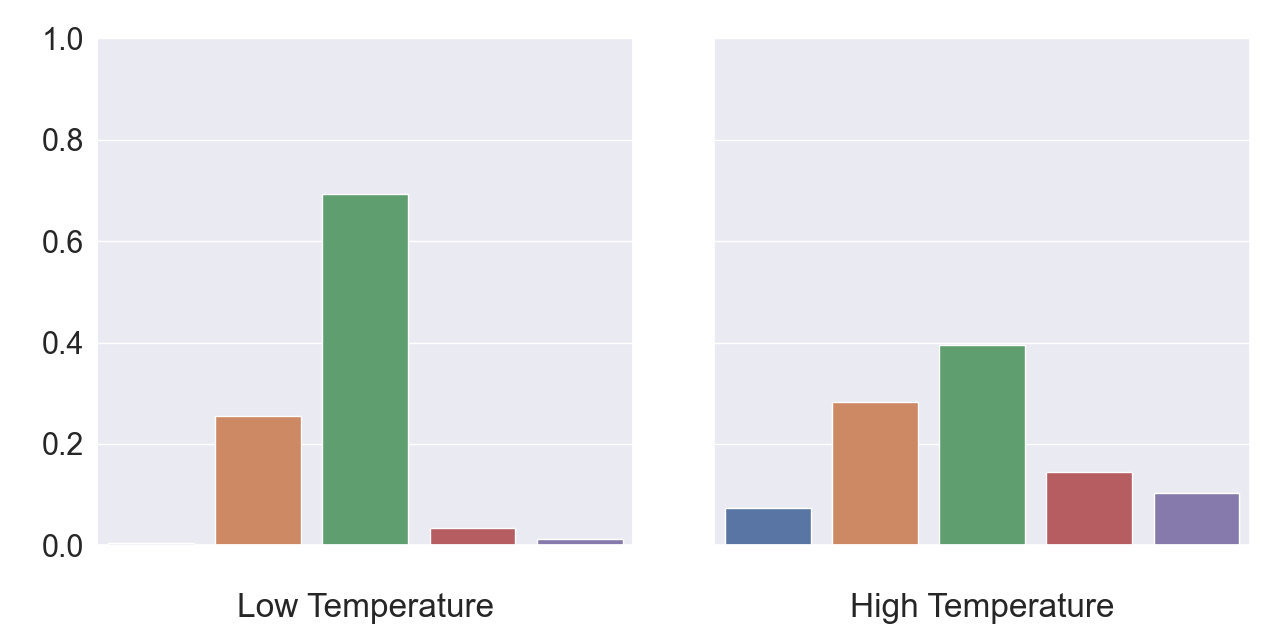
\includegraphics[width=7.5cm]{images/temperature.png}
    \caption{We apply both temperature and softmax to some fixed logits and graph the results. Increasing the temperature increases spread, while decreasing the temperature sharpens the distribution.}
    \label{fig:temperature}
\end{figure}

Temperature scaling is usually implemented by first training a model normally and then determining the optimal value of temperature after the model has finished training. Specifically, the temperature is optimized to minimize the negative log likelihood of the validation set. In practice, temperature scaling works very well, reducing the ECE on Cifar100 of ResNet models to 0.00-0.03.

\subsection{Architectures}
Others have shown that the choice of architecture improves both in-distribution and out-of-distribution calibration \cite{minderer2021revisiting}. In particular, researchers test out seven different models on image classification tasks. They find that two non-convolutional models, vision transformer \cite{dosovitskiy2021image} and MLP-Mixer \cite{tolstikhin2021mlpmixer}, are naturally calibrated with an ECE on ImageNet of between 0.01-0.03. The other five networks had convolutional architectures and had ECE between 0.01-0.09.

Vision transformers are based on the transformer model, a model which was initially developed for NLP. See \href{https://jalammar.github.io/illustrated-transformer/}{\underline{this blogpost}} for an in-depth explanation with illustrations. MLP-Mixer is an architecture which only relies on multi-layer perceptrons (i.e., fully connected layers) to do image classification. Strikingly, despite not leveraging convolutions, both vision transformers and MLP-Mixer perform very well at large scales; MLP-Mixer held an ImageNet accuracy of 87.94\%, and vision transformers an accuracy of 90.45\%.

\subsection{Other Methods}
Other approaches include methods which assign probabilities based on some binning schema \cite{zadrozny2001obtaining, naeini2015obtaining}, methods which leverage ensembles of models \cite{gal2016dropout, lakshminarayanan2017simple}, and methods which train directly on the calibration metrics \cite{kumar2018trainable}. We do not discuss them here, but have provided citations for further exploration.

\section{Out of Distribution Calibration}
Calibration, as measured by metrics like ECE, has mostly been solved on small image datasets through techniques such as temperature scaling. Moreover, significant progress has been made on improving calibration on ImageNet as well. However, general calibration is far from solved. In 2019, researchers from Google/DeepMind identified that calibration significantly degrades on dataset shifts, specifically on corrupted and out-of-distribution data \cite{ovadia2019trust}. Dataset shifts like these represent a large source of error in real-world applications, so it is critical that our models remain calibrated on these inputs. 

\subsection{Uncertainty via Deep Ensembles}
When testing calibration on out-of-distribution data, the Google researchers found that most in-distribution calibration methods, including temperature scaling and some general uncertainty methods \cite{gal2016dropout, guo2017calibration}, perform only marginally better than doing nothing. By far, the strongest baseline method was deep ensembling, a technique which derives uncertainty estimates from ensembling over a population of models \cite{lakshminarayanan2017simple}. 

The method involves training a single model architecture multiple times with different weight initializations. After training, the models' predictions are averaged and used as a probability distribution. Intuitively, averaging over the ensemble filters out the spurious model overconfidences and leaves only confidence scores with which the ensemble largely agrees. For good uncertainty estimates, the population should have at least five models and scaling further to ten or fifteen models provides significant albeit small returns.

The paper also provides one other trick for classification: using adversarial training to smooth out the model predictions. Ablation studies showed that these techniques provide modest improvement over basic ensembling.

\subsection{Prior Networks} % Move to ood detection?
Another approach involves modeling distribution shift explicitly \cite{malinin2018predictive, charpentier2020posterior}. In particular, this line of direction argues that current uncertainty methods are conflating multiple different types of uncertainty. They argue that distribution uncertainty—uncertainty which comes from distribution shift—is different from model uncertainty and data uncertainty. Model uncertainty (also known as \textit{epistemic uncertainty}) arises from the uncertainty in having a limited dataset and not knowing which model is best. Data uncertainty (also known as \textit{aleatoric uncertainty}) is uncertainty inherent in the task which cannot be reduced by improving the model. E.g., if an image is misclassified because the model does not have enough data, that's model uncertainty. If an image is misclassified because it's blurry and inherently uncertain, that's data uncertainty. 

Prior Networks \cite{malinin2018predictive} (and later Posterior Networks \cite{charpentier2020posterior}) distinguish distributional uncertainty from the other two by explicitly model distribution uncertainty using a parameterizable prior distribution. Although the approaches are currently under active development, modeling distributional uncertainty directly is a promising direction and will likely reappear in the future.

\subsection{Exposure to Out of Distribution Examples}
Finally, exposure to out-of-distribution examples (as part of a distribution shift robustness or out-of-distribution detection method) can also improve out-of-distribution calibration. For instance, certain data augmentation techniques can increase both distribution shift robustness and calibration on out-of-distribution images \cite{hendrycks2021pixmix}. Furthermore, some out-of-distribution detection methods also improve out-of-distribution calibration \cite{hendrycks2018deep}. Intuitively, by being exposed to a more diverse set of images, the model naturally becomes more calibrated on out-of-distribution images.

\subsection{Further Research} % A lot of distribution shift specific stuff helps out calibration. E.g., outlier exposure or data augmentation. Also https://openreview.net/pdf?id=ryiAv2xAZ
% Maybe the argument should be that ood calibration is merging with dsr or ood detection? (Reference papers in the previous section
As the problem of out-of-distribution calibration is relatively new, there do not exist many approaches beyond deep ensembles and prior networks for tackling this problem. Some work has established that architecture and model size affects out-of-distribution calibration \cite{minderer2021revisiting}. However the analysis has been relatively brief and leave many questions unanswered. E.g., how does pretraining affect out-of-distribution calibration? Why do certain distribution shifts have calibration and accuracy correlated, whereas other shifts do not? How does architecture and model size affect calibration and why? The field, as it stands, waits for these simple problems to be explored.

\section{Conclusion}
Having well-calibrated models which know their own uncertainties is essential to the safe deployment of machine learning systems. In this chapter, we have discussed how modern deep neural networks may not be well-calibrated, how researchers are able to quantify this miscalibration, and how researchers usually address in-distribution calibration. Finally, we discussed calibration on out-of-distribution or corrupted inputs as well as a few promising approaches.

\bibliographystyle{plain}
\bibliography{reference}

\end{document}
